\chapter{Basic Concepts in Computer Networking}
\section{Networking Stack}
\begin{definitionbox}{Application Layer}
    Applications send and recieve data in a format they specify. Implementations detais of \textbf{OS}, \textbf{packet types}, \textbf{network} setups and hardware models are abstracted away.
    \\
    \\ Applications use protocols which define structure of data (requests and responses), as well as port numbers and other conventions.
    \begin{center}
        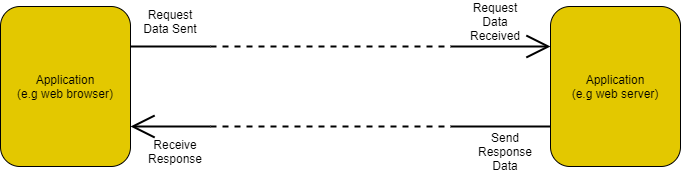
\includegraphics[width=0.8\textwidth]{basic_concepts_and_osi/images/application layer.png}
    \end{center}
\end{definitionbox}
\begin{examplebox}{World Wide Web}
    Part of the internet, invested by Tim Berners-Lee while working at CERN. It uses \textbf{HTTP}(HyperText Transfer Protocol). Early versions use plain text (newer \& more advanced no longer always true).
    \begin{center}
        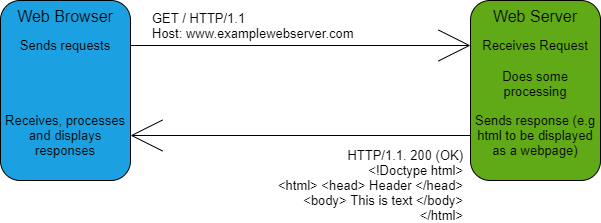
\includegraphics[width=0.8\textwidth]{basic_concepts_and_osi/images/world wide web.png}
    \end{center}
    \textbf{HTTP} exists in the application layer of the \textbf{TCP/IP} stack. The level of abstraction on which we consider protocols, agreements and transfer of application data.
\end{examplebox}

\begin{definitionbox}{Transport Layer}
    Establishes basic data channels, taking data to be sent or being recieved and converting to/from data packets. Networking can be:
    \begin{tabular}{l l l}
        \textbf{Connection-oriented} & \textbf{TCP} - Transmission Control Protocol & Packets not acknowledged to have been received are re-sent. \\
        \textbf{Connectionless}      & \textbf{UDP} - User Datagram Protocol        & No checking, packets sent once, more performant.            \\
    \end{tabular}
    \begin{center}
        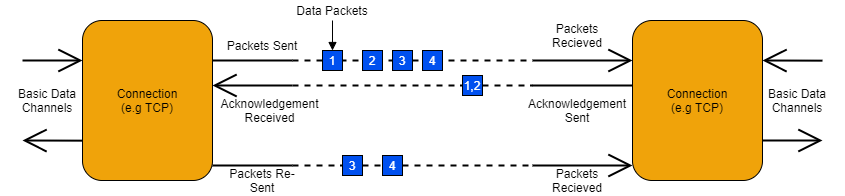
\includegraphics[width=0.8\textwidth]{basic_concepts_and_osi/images/transport layer.png}
    \end{center}
\end{definitionbox}

\begin{definitionbox}{Network Layer}
    The internet protocol is used to add \textbf{IP Addresses} and other information to packets, and then route them through a mesh network of hosts to reach the destination. The path taken frequently changes and is per-packet.
    \begin{center}
        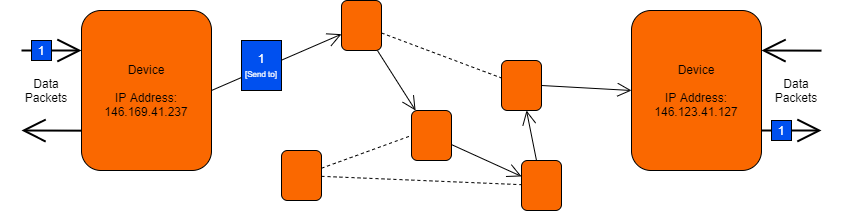
\includegraphics[width=0.8\textwidth]{basic_concepts_and_osi/images/network layer.png}
    \end{center}
\end{definitionbox}

\begin{definitionbox}{Data Link Layer}
    \textbf{NIC} (network Interface Controller) hardware controlling communication over standards to allow physical communication of data (e.g ethernet, wifi, bluetooth, coaxial cable) to transfer data (packets) between devices.
    \begin{center}
        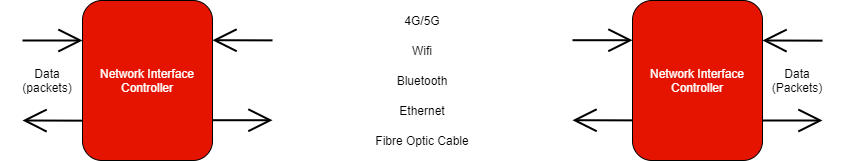
\includegraphics[width=0.8\textwidth]{basic_concepts_and_osi/images/data link layer.png}
    \end{center}
\end{definitionbox}

\begin{definitionbox}{Physical Layer}
    The actual hardware transferring data.
    \begin{itemize}
        \setlength\itemsep{0em}
        \item Fibre-Optic cable
        \item Twisted-pair copper cable
        \item coaxial cable
        \item wireless links (wifi: $802.11$, bluetooth)
    \end{itemize}
\end{definitionbox}

\section{Internet Structure}

\begin{definitionbox}{Host/End System}
    A computer system that is the source, or destination of communication.

    \begin{tabular}{l p{.8\textwidth}}
        \textbf{Smartphone}           & Send and receives data (e.g to browse internet) \\
        \textbf{Home Security System} & To send and receive security footage            \\
    \end{tabular}

    \begin{center}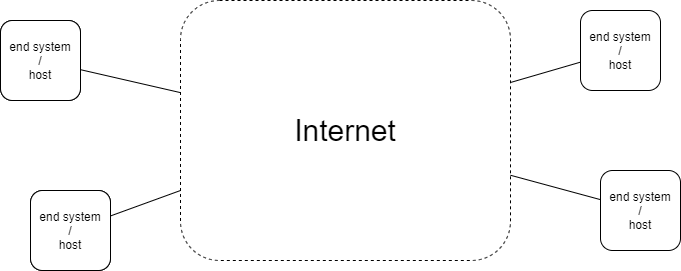
\includegraphics[width=0.7\textwidth]{basic_concepts_and_osi/images/host.png}\end{center}
\end{definitionbox}

\begin{center}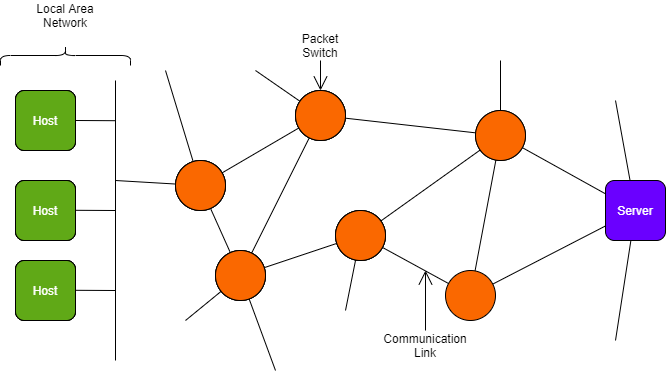
\includegraphics[width=\textwidth]{basic_concepts_and_osi/images/basic internet structure.png}\end{center}

Some simple terms (for now):
\begin{center}
    \begin{tabular}{l p{0.8\textwidth}}
        \textbf{Packet Switch}      & A \textbf{Data Link Layer} switch or router (routes data through a network)                         \\
        \textbf{Communication Link} & A connection between packet switches and/or end systems (hosts).                                    \\
        \textbf{Route}              & A sequence of switches a packet traverses to go from source to destination.                         \\
        \textbf{Protocol}           & A standard concerning the control and format of sending and receiving data to and from end systems. \\
    \end{tabular}
\end{center}

\section{Packet Switching}
\begin{minipage}[t]{0.48\textwidth}
    \centerline{\textbf{Packet Switching}}
    \begin{itemize}
        \setlength\itemsep{0em}
        \item Data is split into packets which are independently routed through the network.
        \item Switches \& routers use packet information, and network status to determine which next router/end system to forward a packet on to.
        \item If any links in the network become slow or disconnected, packets are rerouted.
        \item No setup cost.
        \item Processing cost associated with forwarding each packet.
        \item Space cost associated with containing independent information in each and every packet.
        \item Quality of service is difficult to guarantee (no connection, processing and switching overhead, others can start using links as no reservation).
        \item High network resource utilisation (can send packets different routes in parallel, two connections can work on shared communication links)
    \end{itemize}
    \textbf{Example}\dots The internet.
\end{minipage}
\hfill
\begin{minipage}[t]{0.48\textwidth}
    \centerline{\textbf{Circuit Switching}}
    \begin{itemize}
        \setlength\itemsep{0em}
        \item At the start of a connection, a path is specified and connected.
        \item Connection stays on the path for the entire duration of the communication.
        \item High setup cost to create path.
        \item No processing or space cost as data can be sent straight down the link.
        \item If the link becomes slow (over-saturated) or breaks a new link must be obtained (slow).
        \item Network Resources are reserved at connection start, so quality of service is guaranteed.
        \item Reservation of a route leads to inefficient network resource utilisation.
    \end{itemize}
    \textbf{Example}\dots Older telecommunication systems (landline).
\end{minipage}
\begin{sidenotebox}{Telephone Network}
    The old telephone network (modern is digital, Voice over IP) ius a circuit switched network. A circuit (path through the network) is connected and maintained for the call's duration.
\end{sidenotebox}

\section{Internet Protocol Stack}
\begin{definitionbox}{Communication Protocol}
    A network protocol is an established set of rules that determine how data is transmitted between different devices. (e.g describe layout and meaning of packets and the order they should be sent).
    \begin{center}
        \begin{tabular}{l p{0.8\textwidth}}
            \textbf{Phase} & \textbf{Description}                                                                 \\
            Handshake      & Establishes identities, and the context to begin the communication.                  \\
            Conversation   & Communication, exchanging data in the format \& way specified by the protocol.       \\
            Closing        & Terminates the conversation, performing any necessary cleanup/notification to other. \\
        \end{tabular}
    \end{center}
\end{definitionbox}

\section{Hybrid 5-Layer Model}
For this module we consider the 5 layer model of the networking stack.
\begin{center}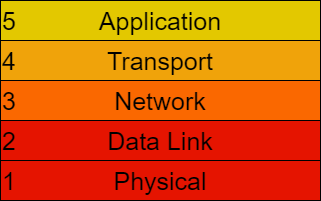
\includegraphics[width=0.4\textwidth]{basic_concepts_and_osi/images/internet protocol stack.png}\end{center}
\begin{center}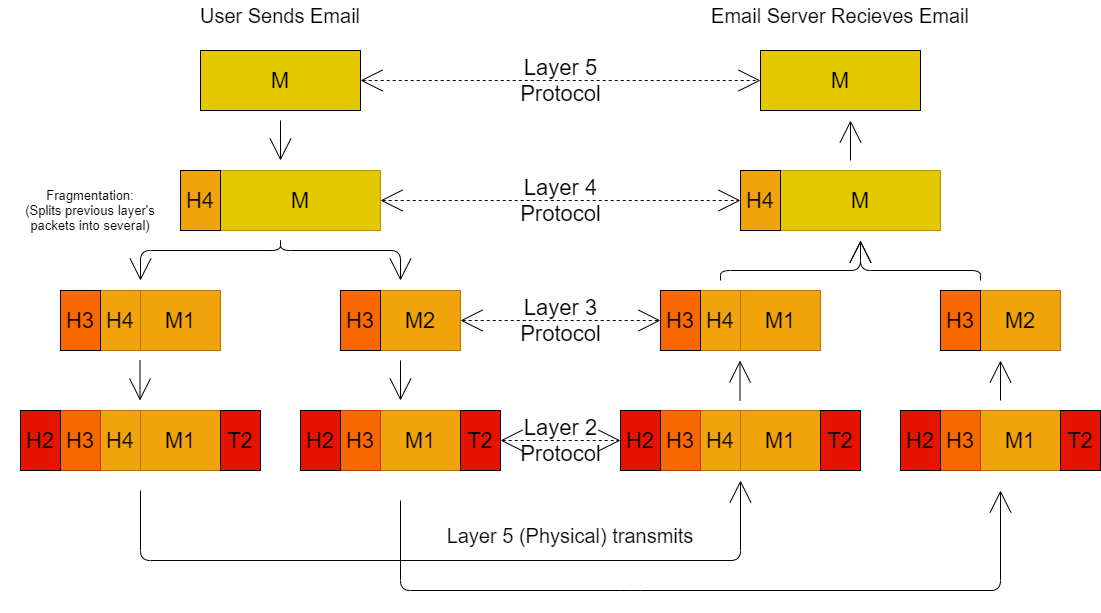
\includegraphics[width=\textwidth]{basic_concepts_and_osi/images/layers working.png}\end{center}
For example when communication through other switches:
\begin{center}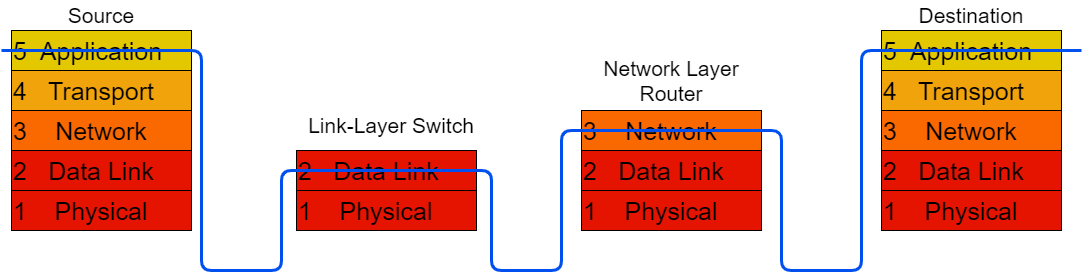
\includegraphics[width=\textwidth]{basic_concepts_and_osi/images/layer communication.png}\end{center}
\begin{sidenotebox}{Alternative Models}
    In this course the 5 layer model is used. The reason being that Dr Gkoutzis claims it is the best. I ( \& you) have no reason to doubt this.
    \\
    \\ There is also:
    \\ \begin{minipage}[t]{0.48\textwidth}
        \centerline{\textbf{7-Layer OSI}}
        \begin{center}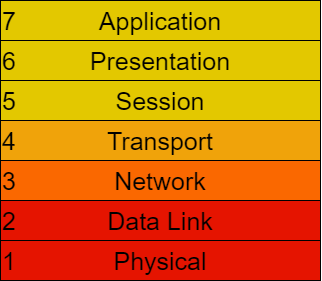
\includegraphics[width=0.9\textwidth]{basic_concepts_and_osi/images/7-layer osi.png}\end{center}
    \end{minipage}
    \begin{minipage}[t]{0.48\textwidth}
        \centerline{\textbf{4-Layer TCP/IP}}
        \begin{center}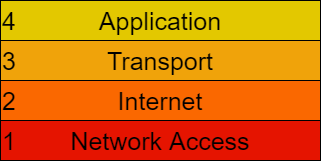
\includegraphics[width=0.9\textwidth]{basic_concepts_and_osi/images/4-layer tcp ip.png}\end{center}
    \end{minipage}
\end{sidenotebox}

\begin{definitionbox}{Service}
    A set of primitives that the layer provides to the layer above. For example the \textbf{Transport Layer} packeting the data sent from the application layer.
\end{definitionbox}

\section{Internet Protocol Design}
When designing a protocol, one must consider:

\begin{tabular}{l p{.8\textwidth}}
    \textbf{Addressing}            & How to denote intended recipient.                                                      \\
    \textbf{Error Control}         & Detection and possible correction of inevitable transmission errors.                   \\
    \textbf{Flow Control}          & Prevent fast sender \textit{swamping} slow receiver.                                   \\
    \textbf{Demulti/Multi-plexing} & Supporting parallel communications.                                                    \\
    \textbf{Routing}               & How to route packets to destination via best route with low processing/space overhead. \\
\end{tabular}

Most \textbf{network layers} have both connection-oriented and connection-less protocols:
\begin{center}
    \begin{tabular}{l p{0.8\textwidth}}
        \textbf{Connection-oriented} & Setup Connection with client, transmit data over channel. (e.g cirtcuit switch, TCP on IP)                               \\
        \textbf{Connectionless}      & Send data to destination address, no formal connection created (\textit{postal mode}). (e.g packet switching, UDP on IP) \\
    \end{tabular}
\end{center}

\subsection{Application Layer Protocols}
\begin{tabular}{l p{.8\textwidth}}
    \textbf{Traditional}  & Name Services (DNS), Email (SMTP), FTP, Telnet, SSH, HTTP/S                                                                     \\
    \textbf{Modern}       & Middleware to support distributed systems (Java RMI, Apache Thrift, Google Protocol Buffers - used for sending serialized data) \\
    \textbf{High Level}   & e-commerce, banking (visa) etc.                                                                                                 \\
    \textbf{Peer-to-peer} & BitTorrent, skype (old protocol)                                                                                                \\
\end{tabular}

\subsection{Transport Layer}
Offers both connection-oriented and connection-less protocols.
\begin{itemize}
    \setlength\itemsep{0em}
    \item Often provides network interface through sockets (e.g \textbf{UNIX} sockets).
    \item Provides support for secure connections.
    \item Support for \textbf{datagrams} (unreliable but fast per-message basis sending - connectionless, e.g \textbf{UDP}).
    \item Provides mechanisms to prevent fast senders overwhelming slow receivers.
\end{itemize}

\subsubsection*{Network Layer}
Describes how routing and congestion is done.
\begin{itemize}
    \setlength\itemsep{0em}
    \item Determining best route.
    \item Dealing with router unreliability (e.g connection goes down).
    \item Supporting multicasting/broadcasting.
    \item Dealing with packet dropping (e.g when a router is overloaded).
\end{itemize}

\begin{sidenotebox}{Multicasting}
    Sending information to many recipients from a single source. Useful to reduce network traffic, for example a CCTV system sending a single video stream to be recieved by many screens, backups.
\end{sidenotebox}

\subsection{Data Link Layer}
Reducing, detecting and rectifying bit transmission layers.
\begin{itemize}
    \setlength\itemsep{0em}
    \item Adding parity bits, checksum (e.g Cyclic Redundancy Check).
    \item Specifying how computers can share a common channel (\textbf{MAC} (Media Access Control) addresses).
    \item Specifying how network connects together (e.g Ethernet, FDDI (Fibre Distributed Data Interface)), and token rings (one holds token and listens at a time)
\end{itemize}

\subsection{Physical Layer}
Describe transmission of raw bits in terms of mechanical, electrical, optical means.
\\
\\ e.g set $0: +4V, 1: -3V$ change at frequency of $20KHz$.

\section{Network Performance}

\subsection*{Digital Units}
\begin{minipage}[t]{0.3\textwidth}
    \[\times 1000\]
    \begin{center}
        \begin{tabular}{l l l}
            \textbf{Term} & \textbf{Bytes}            \\
            KiloByte      & KB             & $1000$   \\
            MegaByte      & MB             & $1000^2$ \\
            GigaByte      & GB             & $1000^3$ \\
            TeraByte      & TB             & $1000^4$ \\
            PetaByte      & PB             & $1000^5$ \\
            ExaByte       & EB             & $1000^6$ \\
            ZettaByte     & ZB             & $1000^7$ \\
            YottaByte     & YB             & $1000^8$ \\
        \end{tabular}
    \end{center}
\end{minipage}
\hfill
\begin{minipage}[t]{0.3\textwidth}
    \[\times 1000\]
    \begin{center}
        \begin{tabular}{l l l}
            \textbf{Term} & \textbf{Bits}            \\
            Kilobits      & Kb            & $1000$   \\
            Megabits      & Mb            & $1000^2$ \\
            Gigabits      & Gb            & $1000^3$ \\
            Terabits      & Tb            & $1000^4$ \\
            Petabits      & Pb            & $1000^5$ \\
            Exabits       & Eb            & $1000^6$ \\
            Zettabits     & Zb            & $1000^7$ \\
            Yottabits     & Yb            & $1000^8$ \\
        \end{tabular}
    \end{center}
\end{minipage}
\hfill
\begin{minipage}[t]{0.3\textwidth}
    \[\times 1024\]
    \begin{center}
        \begin{tabular}{l l l}
            \textbf{Term} & \textbf{Bytes}            \\
            KibiByte      & KB             & $1024$   \\
            MebiByte      & MB             & $1024^2$ \\
            GibiByte      & GB             & $1024^3$ \\
            TebiByte      & TB             & $1024^4$ \\
            PebiByte      & PB             & $1024^5$ \\
            ExbiByte      & EB             & $1024^6$ \\
            ZebibByte     & ZB             & $1024^7$ \\
            YobiByte      & YB             & $1024^8$ \\
        \end{tabular}
    \end{center}
\end{minipage}

\subsection{Speed and Capacity}
\begin{center}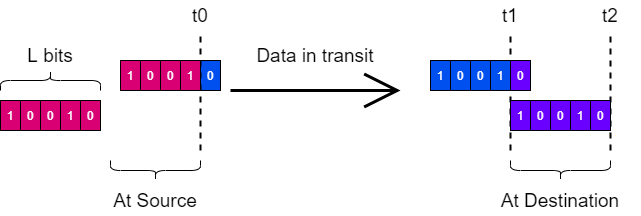
\includegraphics[width=0.8\textwidth]{basic_concepts_and_osi/images/network performance.png}\end{center}
\begin{center}
    \begin{tabular}{l l c}
        \textbf{Term}          & \textbf{Description}                                               & \textbf{Formula}            \\
        \hline
        \\
        \textbf{Throughput}    & Total data received per time (link bandwidth).                     & $R = \cfrac{L}{t_2 - t_1}$  \\
        \\
        \hline
        \\
        \textbf{Latency}       & Time taken for a single bit to be transmitted (propagation delay). & $d = t_1 - t_0$             \\
        \\
        \hline
        \\
        \textbf{Packetization} & Time per bit to be received (transmission delay).                  & $\cfrac{L}{R}$              \\
        \\
        \hline
        \\
        \textbf{Bandwidth}     & Maximum possible throughput.                                       &                             \\
        \\
        \hline
        \\
        \textbf{Transfer Time} & Send time per bit                                                  & $\Delta = d + \cfrac{L}{R}$ \\
    \end{tabular}
\end{center}

\begin{examplebox}{Small Email}
    We are transfering a file from London $\to$ Edinburgh.
    \[\begin{matrix}
            L = 4KB & d = 500ms & R = 1MB/s
        \end{matrix}\]
    What is the transfer time ($\Delta$)?
    \\
    \\ To get transmission delay. $\cfrac{4KB}{1MB/s} = \cfrac{4}{1000}s = 4ms$
    \\ Hence transfer time is: $500ms + 4ms = 504ms$.
\end{examplebox}
\begin{examplebox}{Big File}
    We are transfering a large file:
    \[\begin{matrix}
            L = 700MB & d = 500ms & R = 1MB/s
        \end{matrix}\]
    Find the transfer time ($\Delta$).
    \\
    \\ To get transmission delay: $\cfrac{700MB}{1MB/s} = 700s$
    \\ Hence transfer time is: $500ms + 700s = 700.5s$
\end{examplebox}

\subsection{Processing Delay}
Processing delay $d_{proc}$:
\begin{itemize}
    \setlength\itemsep{0em}
    \item Check for bit errors.
    \item Determine output link.
    \item Negligible (<msec).
\end{itemize}
Queueing delay $d_{queue}$:
\begin{itemize}
    \setlength\itemsep{0em}
    \item time waiting at output link for transmission.
    \item If link is congested, packet might be queued for a long time before being sent.
    \item If in queue too long, packet may be dropped.
\end{itemize}
\[\begin{matrix}
        R: \text{ link bandwidth(bps)} & L: \text{ packet length (bits)} & a: \text{ average packet arrival rate} & \cfrac{L \times a}{R}: \text{ traffic intensity} \\
    \end{matrix}\]
\[\text{Delay } = \begin{cases}
        \text{small} & \cfrac{L \times a}{R} \approx 0 \\
        \text{large} & \cfrac{L \times a}{R} \to 1     \\
        \infty       & \cfrac{L \times a}{R} > 1       \\
    \end{cases}\]
If more work is arriving that can be processed, the delay becomes infinite (and packets will likely be dropped).
